\documentclass{beamer}             % pour version presentation
% \documentclass[handout]{beamer}  % pour version imprimable

% \usepackage[french]{babel}

\usepackage{ragged2e}
\usepackage{epsf}
\usepackage{graphicx} 
\usepackage{listings}
\usepackage{calc,tikz}
\usetikzlibrary{calc,tikzmark}

\usepackage{pifont}
\usepackage{booktabs}

\mode<presentation>{
		
 	\usetheme{ARBITRAGE}
	\setbeamercovered{transparent}
}


% To have slides without headlines
% makeatletter permet a @ d'etre regarde comme la lettre, ce qui
% n'est pas le defaut de latex
% makeatother remet ce defaut latex

\makeatletter
    \newenvironment{withoutheadline}{
        \setbeamertemplate{headline}[default]
        \def\beamer@entrycode{\vspace*{-\headheight}}
    }{}
\makeatother


%\title[Federated ILP]{%
%  The Ariac -- Arbitrage Project \\*[1em]
%  On Federated Learning}
%\author[JMJ -- ILI -- WVA]{%
%  J.-M. Jacquet, I. Linden, W. Vanhoof}
%\institute[UNamur]{University of Namur}
%\date{February 8th 2022}
\title[Federated ILP]{%
  Inductive logic programming \\*[1em]
  In Federated Learning}
\author[SJ -- JMJ -- ILI -- WVA]{%
S. Jacquet,  J.-M. Jacquet, I. Linden, W. Vanhoof}
\institute[UNamur]{University of Namur}
\date{February 21st 2022}

% \logo{
\includegraphics[height=0.75cm]{theme/LogoUN.eps}}
% \titlegraphic{
\includegraphics[height=1.25cm]{theme/LogoUN.eps}}

%\logo{
\includegraphics[height=0.75cm]{LogoUN.pdf}}
% \titlegraphic{
\includegraphics[height=1.25cm]{LogoUN.pdf}}

%=======================================================================%
%                                                                       % 
%                               Frames                                  %
%                                                                       % 
%=======================================================================%



\begin{document}

%-------------------------------------------------------------%

\begin{frame}[plain]

\titlepage

\end{frame}

% ----------------------------------------------------------- %

\begin{withoutheadline}
\begin{frame}

\frametitle{Machine learning in a picture}

\begin{center}
% \setlength{\unitlength}{1cm}
\setlength{\unitlength}{0.5cm}
% \begin{picture}(10,15)(0,-3.5)
\begin{picture}(10,15)(0,-2.5)

\put(5,5){%
\begin{picture}(5,5)(3,-1)

\put(0,0){\line(1,0){5}}
\put(0,0){\line(0,1){5}}
\put(0,5){\line(1,0){5}}
\put(5,0){\line(0,1){5}}

\put(2.5,2.5){\makebox(0,0){\begin{tabular}{c}
Learning \\Algo
\end{tabular}}}

\put(-3.5,2.5){\makebox(0,0){\shortstack{$(d_1,r_1)$\\$(d_2,r_2)$\\\ldots\\\mbox{ }\\Rep}}}
\put(7,2.5){%
\begin{picture}(3,2)(0,1)
\put(0,0){\line(1,0){3}}
\put(0,0){\line(0,1){2}}
\put(0,2){\line(1,0){3}}
\put(3,0){\line(0,1){2}}

\put(1.5,1){\makebox(0,0){Model}}

\end{picture}}

\put(-1.5,2.5){\vector(1,0){1}}
\put(5.5,2.5){\vector(1,0){1}}

\end{picture}}

\put(5,-1){%
\begin{picture}(4,4)(2.5,0)

\put(0,0){\line(1,0){4}}
\put(0,0){\line(0,1){4}}
\put(0,4){\line(1,0){4}}
\put(4,0){\line(0,1){4}}

\put(2,2){\makebox(0,0){\begin{tabular}{c}
Model
\end{tabular}}}

\put(-2,2){\makebox(0,0){$d$}}
\put(6,2){\makebox(0,0){$r$}}

\put(-1.5,2){\vector(1,0){1}}
\put(4.5,2){\vector(1,0){1}}

\end{picture}}


\end{picture}
\end{center}

\end{frame}
\end{withoutheadline}

%---------------------------------------------------------------------------------------%
 
\begin{withoutheadline}
\begin{frame}

\frametitle{Typical applications}
  
\begin{center}
\begin{tikzpicture}

\node (ml) at (0,5) {
\includegraphics[height=5em]{images/machine_learning.png}} ;

\node (recom) at (-4,0) {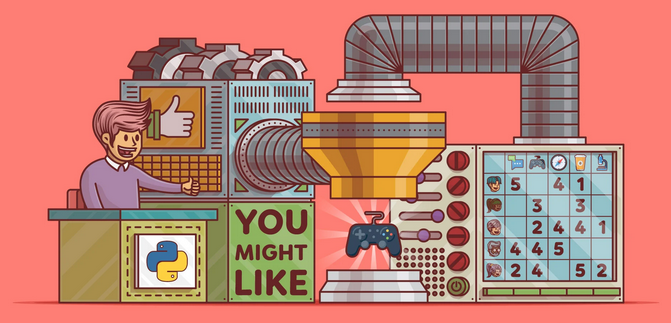
\includegraphics[height=4em]{images/recommendation.png}} ;

\node (img) at (4,0) {
\includegraphics[height=4em]{images/Automated-Image-Recognition.jpg}} ;

\node (data) at (0,0) {
\includegraphics[height=4em]{images/data_analysis.png}} ;

\draw[-latex] (ml) -- (recom);
\draw[-latex] (ml) -- (img);
\draw[-latex] (ml) -- (data); 

\end{tikzpicture}
\end{center}


\end{frame}
\end{withoutheadline}

%---------------------------------------------------------------------------------------%

\begin{withoutheadline}
\begin{frame}

\frametitle{Two kinds of representation}

\begin{center}
\begin{tikzpicture}

\node (declvsproc) at (0,5) {
\includegraphics[height=6em]{images/decl_vs_proc.png}} ;

\node (ilp) at (-4,2) {
\includegraphics[height=5em]{images/ilp.png}} ;
\node (decision) at (0,0) {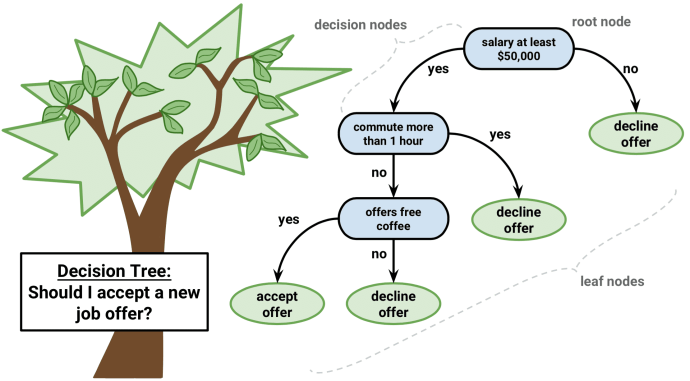
\includegraphics[height=5em]{images/decision_tree.png}} ;
\node (neural) at (4,2) {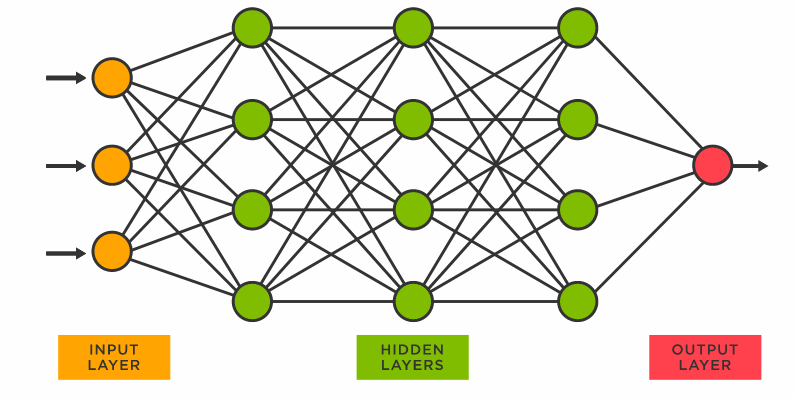
\includegraphics[height=5em]{images/neuralnetwork.png}} ;

\end{tikzpicture}
\end{center}

\end{frame}
\end{withoutheadline}

%---------------------------------------------------------------------------------------%

\begin{withoutheadline}
\begin{frame}[fragile]

\frametitle{Inductive logic programming}

\begin{itemize}
 
\vfill
\pause
\item Given background knowledge

\begin{center}
\begin{minipage}{8.5cm}
\begin{block}{}
\begin{lstlisting}[basicstyle=\scriptsize]
parent(ann,mary).      female(ann).
parent(ann,tom).       female(mary).
parent(tom,eve).       female(eve).
\end{lstlisting}
\end{block}
\end{minipage}
\end{center}

\vfill
\pause
\item Given positive and negative information

\begin{center}
\begin{minipage}{8.5cm}
\begin{block}{}
\begin{lstlisting}[basicstyle=\scriptsize]
+ daughter(mary,ann).    - daughter(tom,ann).
+ daughter(eve,tom).     - daughter(tom,eve).
\end{lstlisting}
\end{block}
\end{minipage}
\end{center}

\vfill
\pause
\item Induce relations
\begin{center}
\begin{minipage}{8.5cm}
\begin{block}{}
\begin{lstlisting}[basicstyle=\scriptsize]
daughter(X,Y) :- parent(Y,X), female(X).
\end{lstlisting}
\end{block}
\end{minipage}
\end{center}

\vfill
\end{itemize}

\end{frame}
\end{withoutheadline}

%---------------------------------------------------------------------------------------%

\begin{withoutheadline}
\begin{frame}

\frametitle{Basic strategy}

\vfill
\hspace*{-1.1cm}
\begin{tikzpicture}

  \node (top) at (0,6) {\scriptsize \begin{tabular}{c}
                 daughter(X,Y) :- true \\ \textit{\tiny (p=2, n=2, f=-2)}
                 \end{tabular}} ;

\only<2->{
  \node (p) at (-4,4) {\scriptsize \begin{tabular}{c}
      daughter(X,Y) :- parent(Y,X). \\ \textit{\tiny (p=2, n=1, f=0)}
  \end{tabular}} ;
}

\only<4->{
  \node (e) at (0,4.5) {\scriptsize daughter(X,Y) :- ...} ;
}

\only<3->{
  \node (f) at (4,4) {\scriptsize \begin{tabular}{c}
      daughter(X,Y) :- female(X). \\ \textit{\tiny (p=2, n=1, f=-1)}
  \end{tabular}} ;
}

\only<5->{
  \node (c) at (-4,1.5) {\scriptsize \begin{tabular}{c}
      daughter(X,Y) :- parent(Y,X), female(X). \\ \textit{\tiny (p=2, n=0, f=2)}
  \end{tabular}} ;
}

\only<6->{
  \node (w) at (2,2.5) {\scriptsize \begin{tabular}{c}
      daughter(X,Y) :- parent(Y,X), female(Y). \\ \textit{\tiny (p=2, n=2, f=0)}
  \end{tabular} } ;
}

\only<2->{\draw[-latex] (top) -- (p); }
\only<4->{\draw[-latex] (top) -- (e);  }
\only<3->{\draw[-latex] (top) -- (f);  }
\only<5->{\draw[-latex] (p) -- (c);  }
\only<6->{\draw[-latex] (p) -- (w);  }

\end{tikzpicture}

\vfill
\only<7->{
\begin{center}
\begin{minipage}{6cm}
\begin{block}{\centering Key features}
\centering Incremental \& theory-based
\end{block}
\end{minipage}
\end{center}
}

\vfill
\end{frame}
\end{withoutheadline}

%---------------------------------------------------------------------------------------%

\begin{withoutheadline}
\begin{frame}

\frametitle{Federated learning}

\hspace*{-0.75cm}
\begin{tikzpicture}

\node (meddata) at (0,0) {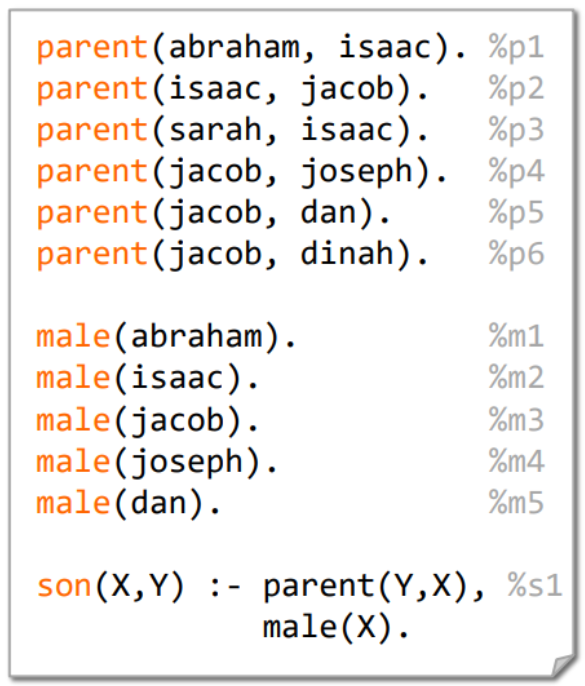
\includegraphics[height=5em]{images/ljocgbpiikbniknb.png}} ;

\node (hi) at (-4,5) {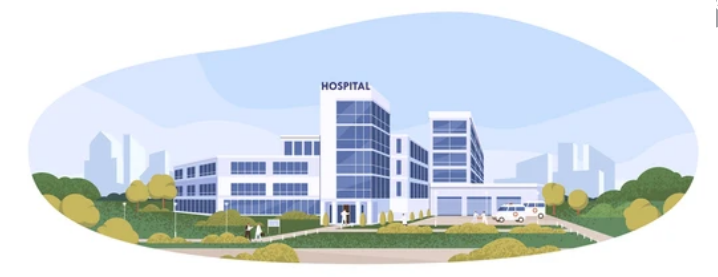
\includegraphics[height=4em]{images/hospital2.png}} ;
\node (hii) at (0,6) {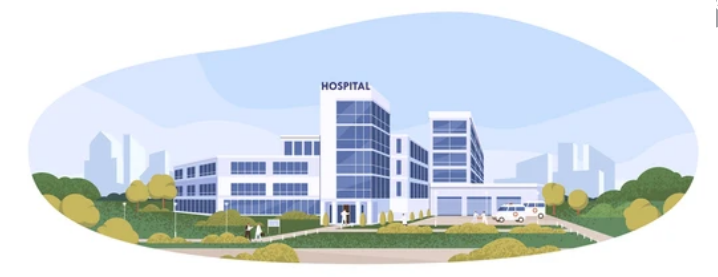
\includegraphics[height=4em]{images/hospital2.png}} ;
\node (hiii) at (4,5) {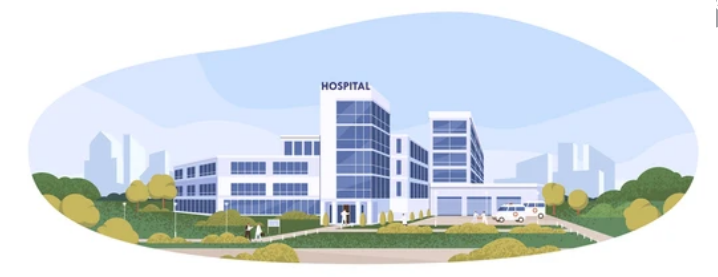
\includegraphics[height=4em]{images/hospital2.png}} ;

\node (clouds) at (0,3) {
\includegraphics[height=5em]{images/clouds2.png}} ;

\draw[-latex] (hi) -- ($(clouds)+(-0.9,0.9)$);
\draw[-latex] (hii) -- (clouds);
\draw[-latex] (hiii) -- ($(clouds)+(0.9,0.9)$);

\draw[-latex] (clouds) -- (meddata);


\only<2->{\node (question) at (0,2.75) {\Large\bf ?};}

\only<3->{\node (ai) at (-4,2.5) {%
\begin{minipage}{4cm}
\setbeamercolor{block title}{bg=blue!30,fg=black}
\begin{block}{Classical solutions}
\begin{itemize}
\item anonymize data \& combine at central node
\item use blockchain technology
\end{itemize}
\end{block}
\end{minipage}
}; }

\only<4->{\node (ai) at (4,2.5) {%
\begin{minipage}{4cm}
\begin{block}{Proposed solution}
\begin{itemize}
\item learn theories locally
\item combine theories at central node
\end{itemize}
\end{block}
\end{minipage}
}; }

\end{tikzpicture}

\end{frame}
\end{withoutheadline}

%---------------------------------------------------------------------------------------%


\end{document}

